\documentclass[12pt, a4paper]{article}

% ─── Paquetes ───────────────────────────────────────────────────────────────
\usepackage[utf8]{inputenc}
\usepackage[T1]{fontenc}
\usepackage[spanish]{babel}
\usepackage[left=2.5cm, right=2.5cm, top=3cm, bottom=3cm]{geometry}
\usepackage{booktabs}
\usepackage{array}
\usepackage{xcolor}
\usepackage{colortbl}
\usepackage{graphicx}
\usepackage{fancyhdr}
\usepackage{titlesec}
\usepackage{pgfplots}
\usepackage{pgfplotstable}
\usepackage{tikz}
\usepackage{multirow}
\usepackage{float}
\usepackage{caption}
\usepackage{parskip}
\usepackage{mdframed}
\usepackage{amsmath}

\pgfplotsset{compat=1.18}
\usetikzlibrary{positioning, shapes.geometric}

% ─── Colores corporativos ────────────────────────────────────────────────────
\definecolor{azulprincipal}{RGB}{0, 70, 127}
\definecolor{azulclaro}{RGB}{210, 228, 245}
\definecolor{grisclaro}{RGB}{245, 245, 245}
\definecolor{verdekpi}{RGB}{39, 174, 96}
\definecolor{rojokpi}{RGB}{192, 57, 43}
\definecolor{amarillokpi}{RGB}{243, 156, 18}
\definecolor{moradokpi}{RGB}{142, 68, 173}

% ─── Encabezado y pie de página ──────────────────────────────────────────────
\pagestyle{fancy}
\fancyhf{}
\fancyhead[L]{\small\color{azulprincipal}\textbf{Imágenes Diagnósticas S.A.}}
\fancyhead[R]{\small\color{azulprincipal}Reporte Mensual de Atención --- Enero 2026}
\fancyfoot[C]{\small\thepage}
\renewcommand{\headrulewidth}{0.4pt}
\renewcommand{\headrule}{\hbox to\headwidth{\color{azulprincipal}\leaders\hrule height \headrulewidth\hfill}}

% ─── Estilo de secciones ─────────────────────────────────────────────────────
\titleformat{\section}
  {\large\bfseries\color{azulprincipal}}
  {\thesection.}{0.5em}{}[\titlerule]
\titleformat{\subsection}
  {\normalsize\bfseries\color{azulprincipal}}
  {\thesubsection.}{0.5em}{}

% ─── KPI box ─────────────────────────────────────────────────────────────────
\newcommand{\kpibox}[3]{%
  \begin{tikzpicture}
    \node[rectangle, rounded corners=4pt, fill=#3,
          minimum width=3.2cm, minimum height=1.6cm, text centered] (box) {};
    \node[above=0.35cm of box.center, anchor=center,
          font=\tiny\bfseries\color{white}] {#1};
    \node[below=0.25cm of box.center, anchor=center,
          font=\large\bfseries\color{white}] {#2};
  \end{tikzpicture}%
}

% ════════════════════════════════════════════════════════════════════════════
\begin{document}
\shorthandoff{<>}

% ── PORTADA ──────────────────────────────────────────────────────────────────
\begin{titlepage}
  \centering
  \vspace*{2cm}
  {\color{azulprincipal}\rule{\linewidth}{1.5pt}}\\[0.4cm]
  {\Huge\bfseries\color{azulprincipal} Reporte Mensual\\[0.3cm] de Atención al Cliente}\\[0.4cm]
  {\color{azulprincipal}\rule{\linewidth}{1.5pt}}\\[1.5cm]
  {\LARGE\color{black} Enero 2026}\\[0.5cm]
  {\large Imágenes Diagnósticas S.A.}\\[0.3cm]
  {\normalsize Canal WhatsApp --- Asignación de Citas}
  \vfill
  {\small Generado automáticamente a partir del sistema de gestión de conversaciones.\\
  Período analizado: 1 -- 30 de Enero de 2026.}
\end{titlepage}

% ── RESUMEN EJECUTIVO ─────────────────────────────────────────────────────────
\section{Resumen Ejecutivo}

Durante el período del 1 al 30 de Enero de 2026
se atendieron un total de \textbf{2845}
conversaciones válidas a través del canal de WhatsApp.

\vspace{0.5cm}
\noindent
\begin{center}
\begin{tabular}{cccc}
  \kpibox{Prom. 1a Respuesta}{30m}{azulprincipal} &
  \kpibox{Satisfaccion Agente}{4.6/5}{verdekpi} &
  \kpibox{Cantidad conversaciones}{2845}{moradokpi} &
  \kpibox{Conv. Agendadas}{34.5\%}{amarillokpi}
\end{tabular}
\end{center}

\vspace{0.3cm}
\begin{mdframed}[backgroundcolor=grisclaro, linecolor=azulprincipal, linewidth=0.8pt]
\small
\textbf{Nota metodologica:} Se excluyeron \textbf{207}
conversaciones de agentes internos y sin primera respuesta registrada.
Se excluyeron ademas \textbf{15} conversaciones
iniciadas en dias festivos.
\end{mdframed}

% ── MÉTRICA 1 — PROMEDIO DIARIO DE CONVERSACIONES ────────────────────────────
\section{Promedio Diario de Conversaciones}

\begin{figure}[H]
\centering
\begin{tikzpicture}
\begin{axis}[
    ybar, bar width=0.6cm,
    width=13cm, height=7cm,
    symbolic x coords={lunes, martes, miercoles, jueves, viernes, sabado, domingo},
    xtick=data,
    x tick label style={font=\small},
    ymin=0,
    ylabel={\small Promedio de conversaciones},
    grid=major, grid style={dashed, gray!30},
    nodes near coords, nodes near coords style={font=\tiny\bfseries},
    fill=azulprincipal, draw=none,
    enlarge x limits=0.1,
]
\addplot coordinates {
  (lunes, 171.0)
  (martes, 151.0)
  (miercoles, 140.75)
  (jueves, 125.5)
  (viernes, 106.8)
  (sabado, 25.25)
  (domingo, 7.0)
};
\end{axis}
\end{tikzpicture}
\caption{Promedio de conversaciones por dia de la semana --- Enero 2026}
\end{figure}

% ── MÉTRICA 2 — MENSAJES POR HORA (CONTACTOS) ────────────────────────────────
\section{Distribucion de Mensajes por Hora}

\begin{figure}[H]
\centering
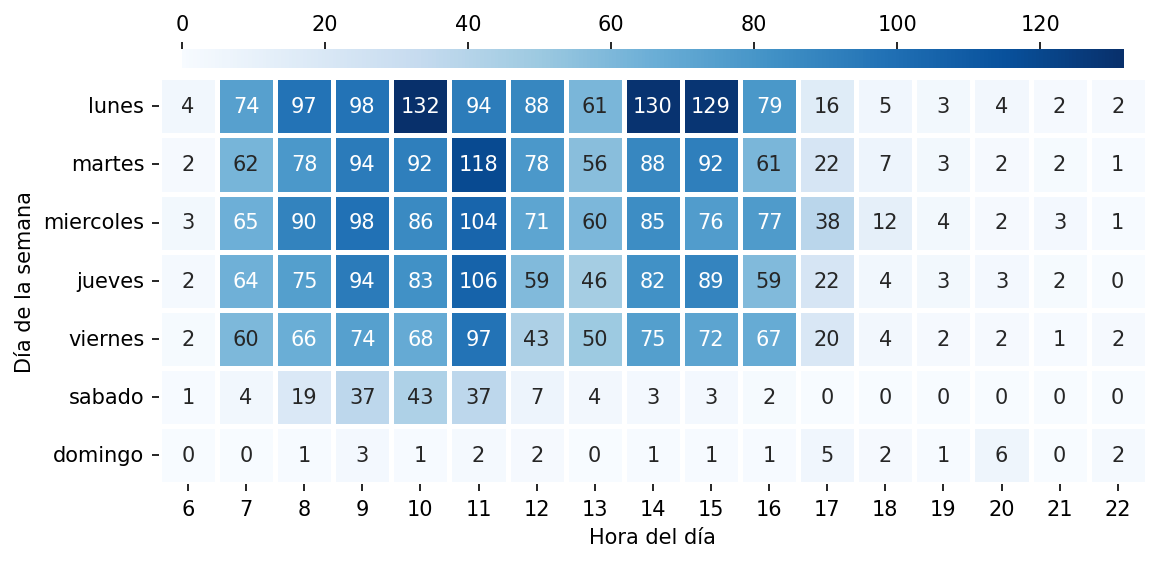
\includegraphics[width=1.1\textwidth]{heatmap_contactos.png}
\caption{Heatmap de mensajes promedio por hora y dia de la semana (contactos)}
\end{figure}

\begin{mdframed}[backgroundcolor=grisclaro, linecolor=azulprincipal, linewidth=0.8pt]
\small Total de mensajes de contactos analizados: \textbf{17723}.
\end{mdframed}

% ── MÉTRICA 3 — MENSAJES POR HORA POR AGENTE ─────────────────────────────────
\section{Productividad de Agentes --- Mensajes por Hora}

\begin{figure}[H]
\centering
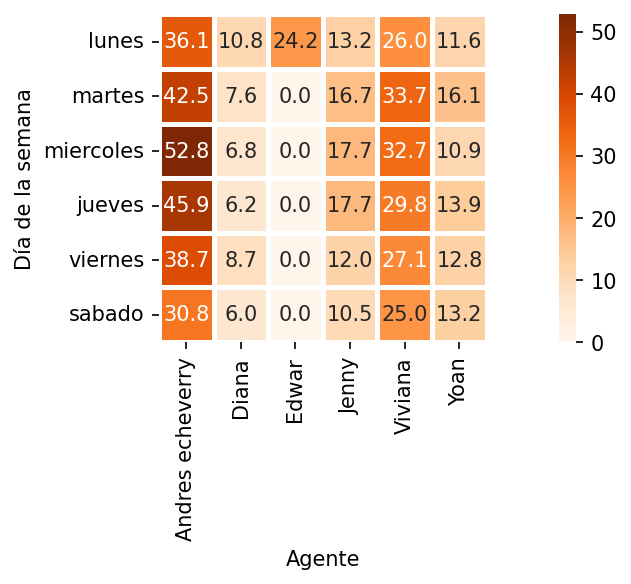
\includegraphics[width=0.85\textwidth]{heatmap_agentes.png}
\caption{Heatmap de mensajes/hora por agente --- Lun--Sab, horario laboral}
\end{figure}

\begin{mdframed}[backgroundcolor=grisclaro, linecolor=azulprincipal, linewidth=0.8pt]
\small\textbf{Criterio horas laborales:} Lunes a viernes = 8 horas, Sabado = 5 horas, Domingo = no laboral.
\end{mdframed}

% ── MÉTRICA 4 — PROMEDIO DE PRIMERA RESPUESTA ────────────────────────────────
\section{Tiempo Promedio de Primera Respuesta}

\begin{figure}[H]
\centering
\begin{tikzpicture}
\begin{axis}[
    ybar, bar width=1.8cm,
    width=10cm, height=7cm,
    symbolic x coords={Con plantilla, Sin plantilla, Total},
    xtick=data,
    x tick label style={font=\small},
    ymin=0,
    ylabel={\small Minutos},
    grid=major, grid style={dashed, gray!30},
    nodes near coords, nodes near coords style={font=\small\bfseries},
    enlarge x limits=0.3,
    fill=azulprincipal, draw=none,
]
\addplot coordinates {
(Con plantilla, 24.78)
(Sin plantilla, 31.48)
(Total, 30.73)
};
\end{axis}
\end{tikzpicture}
\caption{Tiempo promedio de primera respuesta en minutos --- Enero 2026}
\end{figure}

\begin{table}[H]
\centering
\caption{Estadisticos descriptivos --- Tiempo de primera respuesta (minutos)}
\begin{tabular}{lc}
\toprule
\textbf{Estadistico} & \textbf{Valor (min)} \\
\midrule
\rowcolor{azulclaro!40} Minimo         & 0.0 \\
\rowcolor{azulclaro!60} Percentil 25\% & 7.1 \\
\rowcolor{azulclaro!80} Mediana (50\%) & 19.44 \\
\rowcolor{azulprincipal!40} Percentil 75\% & 40.13 \\
\rowcolor{azulprincipal!70} Maximo         & 278.63 \\
\bottomrule
\end{tabular}
\end{table}

\begin{mdframed}[backgroundcolor=grisclaro, linecolor=azulprincipal, linewidth=0.8pt]
\small\textbf{Horario laboral:} Lunes a viernes 07:00--17:00, sabados 08:00--12:00.
Tiempos fuera de horario no se contabilizan.
\end{mdframed}

% ── MÉTRICA 5 — PRIMERA RESPUESTA POR AGENTE ─────────────────────────────────
\section{Tiempo de Primera Respuesta por Agente}

\begin{figure}[H]
\centering
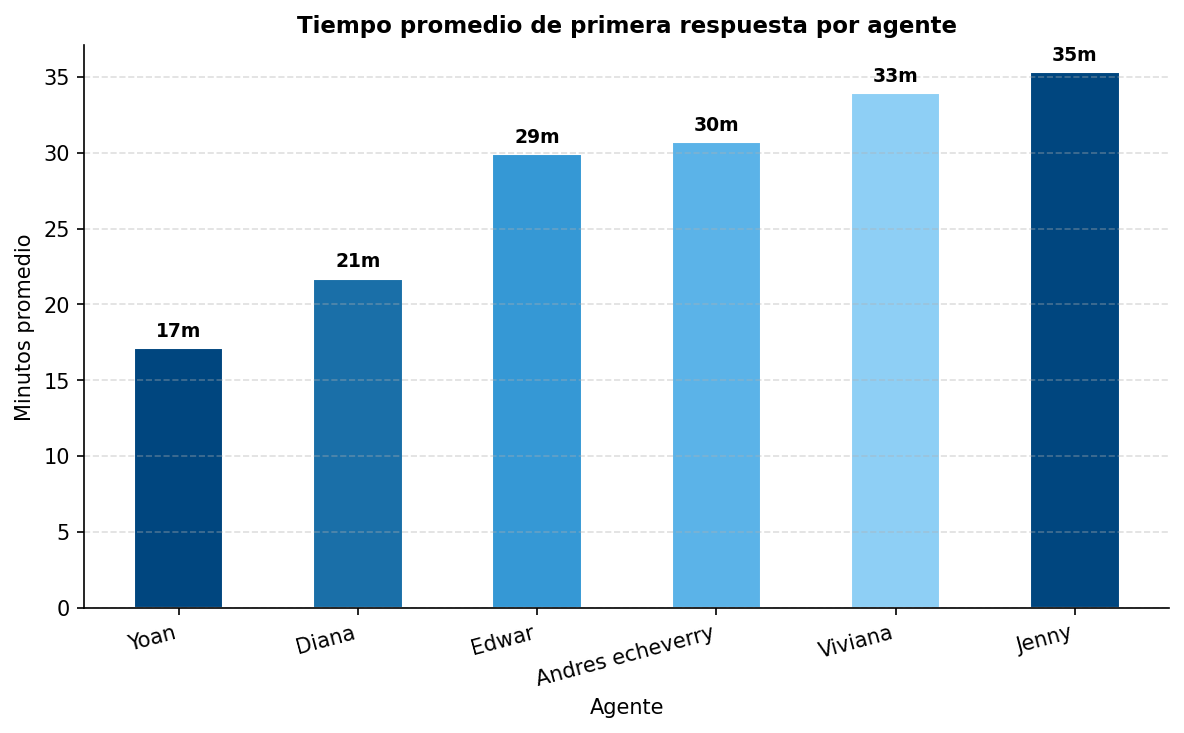
\includegraphics[width=0.85\textwidth]{barras_primera_respuesta_agente.png}
\caption{Tiempo promedio de primera respuesta por agente (minutos) --- mejor a peor}
\end{figure}

% ── MÉTRICA 6 — DURACIÓN DE CONVERSACIONES ───────────────────────────────────
\section{Duracion Promedio de Conversaciones}

\vspace{0.4cm}
\noindent
\begin{center}
\begin{tabular}{cccc}
  \kpibox{Promedio}{32m}{azulprincipal} &
  \kpibox{Mediana}{19m}{azulprincipal} &
  \kpibox{Maximo}{9h 26m}{rojokpi} &
  \kpibox{Minimo}{0m}{verdekpi}
\end{tabular}
\end{center}
\vspace{0.4cm}

\begin{mdframed}[backgroundcolor=grisclaro, linecolor=azulprincipal, linewidth=0.8pt]
\small\textbf{Metodologia:} Suma de tiempos entre el primer mensaje de un bloque de contacto
y la respuesta del agente, dentro del horario laboral.
Total conversaciones analizadas: \textbf{2737}.
\end{mdframed}

% ── MÉTRICA 7 — CONVERSIÓN DE AGENDAMIENTOS ──────────────────────────────────
\section{Conversion de Agendamientos}

\begin{minipage}{0.48\textwidth}
\centering
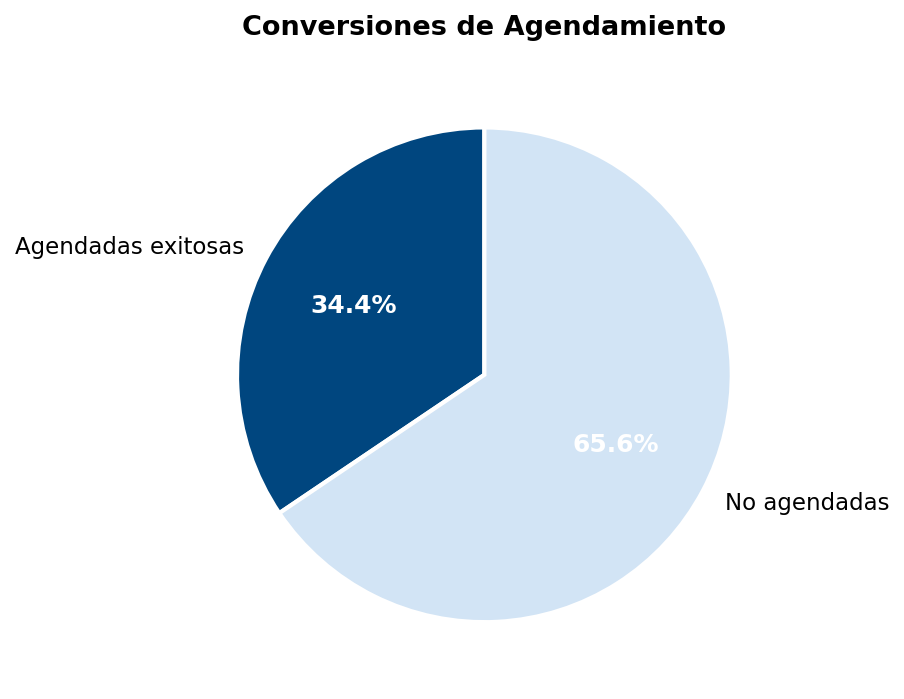
\includegraphics[width=\textwidth]{torta_agendamientos.png}
\end{minipage}
\hfill
\begin{minipage}{0.48\textwidth}
\begin{table}[H]
\centering
\caption{Indicadores de agendamiento}
\begin{tabular}{lc}
\toprule
\textbf{Metrica} & \textbf{Valor} \\
\midrule
Exito sobre iniciadas & 48.69\% \\
Exito sobre no iniciadas & 27.22\% \\
Total conversaciones agendadas & 34.45\% \\
\midrule
Total conversaciones   & 2845 \\
Iniciadas agendamiento & 957 \\
No iniciadas           & 1888 \\
Exitosas               & 980 \\
\bottomrule
\end{tabular}
\end{table}
\end{minipage}

% ── MÉTRICA 8 — SATISFACCIÓN ─────────────────────────────────────────────────
\section{Satisfaccion del Usuario}

\vspace{0.4cm}
\noindent
\begin{center}
\begin{tabular}{cc}
  \kpibox{Satisfaccion Bot}{4.6/5}{verdekpi} &
  \kpibox{Satisfaccion Agente}{4.6/5}{verdekpi}
\end{tabular}
\end{center}
\vspace{0.4cm}

\begin{table}[H]
\centering
\caption{Detalle de calificaciones de satisfaccion}
\begin{tabular}{lcc}
\toprule
\textbf{Indicador} & \textbf{Bot} & \textbf{Agente} \\
\midrule
Promedio (escala 1--5) & 4.6 & 4.6 \\
Total respuestas       & 289 & 289 \\
\bottomrule
\end{tabular}
\end{table}

\begin{mdframed}[backgroundcolor=grisclaro, linecolor=azulprincipal, linewidth=0.8pt]
\small\textbf{Escala:} 1 (muy insatisfecho) a 5 (muy satisfecho).
Solo se consideran sesiones donde el usuario respondio la encuesta.
\end{mdframed}

\end{document}